\documentclass[dvipdfmx,autodetect-engine,titlepage]{jsarticle}
\usepackage[dvipdfm]{graphicx}
\usepackage{ascmac}
\usepackage{fancybox}
\usepackage{listings}
\usepackage{plistings}
\usepackage{itembkbx}
\usepackage{amsmath}
\usepackage{svg}
\usepackage{url}
\usepackage{graphics}
\usepackage{listings,jvlisting}
\usepackage{scalefnt}

\textheight=23cm
\renewcommand{\figurename}{図}
\renewcommand{\tablename}{表}
\newenvironment{code}
{\vspace{0.5zw}\VerbatimEnvironment  
\begin{screen} 
\baselineskip=1.0\normalbaselineskip
 \begin{Verbatim}}
{\end{Verbatim}
\baselineskip=\normalbaselineskip
 \end{screen}\vspace{0.5zw}} 

\title{情報理工学部 SNコース 2回\\
セキュリティ・ネットワーク学実験2\\
NW実験2-5レポート}
\author{2600200443-6\\Yamashita Kyohei\\山下 恭平}
\date{November 17 2021}

\begin{document}

\maketitle

\section{概要}
アプリケーションとポート番号の対応関係をまとめ,さらにウェルノウンポート
について調査しレポートにまとめる。

\section{結果}
lsofコマンドの実行結果に基づいて表を作成した。以下はその実行結果と表である。

\begin{figure}[h]
  \centering
  \caption{OneDrive}
  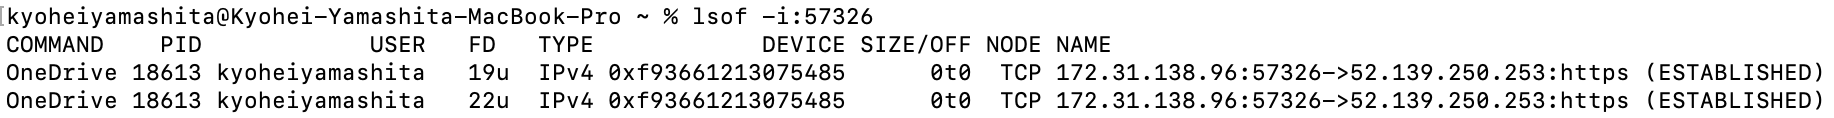
\includegraphics[scale=0.5]{SS1.png}
\end{figure}

\begin{figure}[h]
  \centering
  \caption{Discord}
  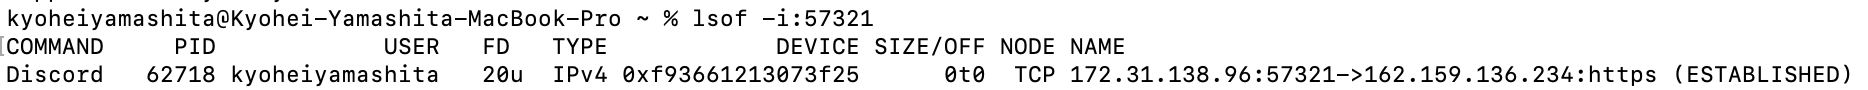
\includegraphics[scale=0.5]{SS2.png}
\end{figure}

\begin{figure}[h]
  \centering
  \caption{LINE}
  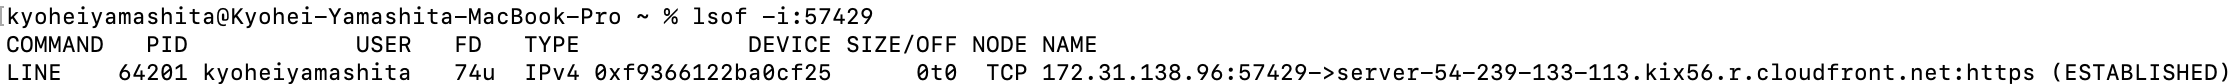
\includegraphics[scale=0.45]{SS3.png}
\end{figure}

\begin{table}[h]
  \centering
  \begin{tabular}{|c|c|c|}
  \hline
  アプリ名     & ポート番号 & PID   \\ \hline \hline
  OneDrive & 57326 & 18613 \\ \hline
  Discord  & 57321 & 62718 \\ \hline
  LINE     & 57429 & 64201 \\ \hline
  \end{tabular}
  \caption{アプリケーション一覧}
  \end{table}

\section{ウェルノウンポートについて}
ウェルノウンポートとは、TCP/IPの通信で利用されるTCPやUDPの0番から65535番まで
のポート番号のうち0番から1023番までのことであり、著名なサービスやプロトコルが
使用するために予約されている。インターネットでサーバを公開するときなどにウェル
ノウンポートが使用されており例えば、HTTPは80番、DNSの53番などがある。

\end{document}

